\section{Introduction}


\begin{figure}
    \centering
    \frame{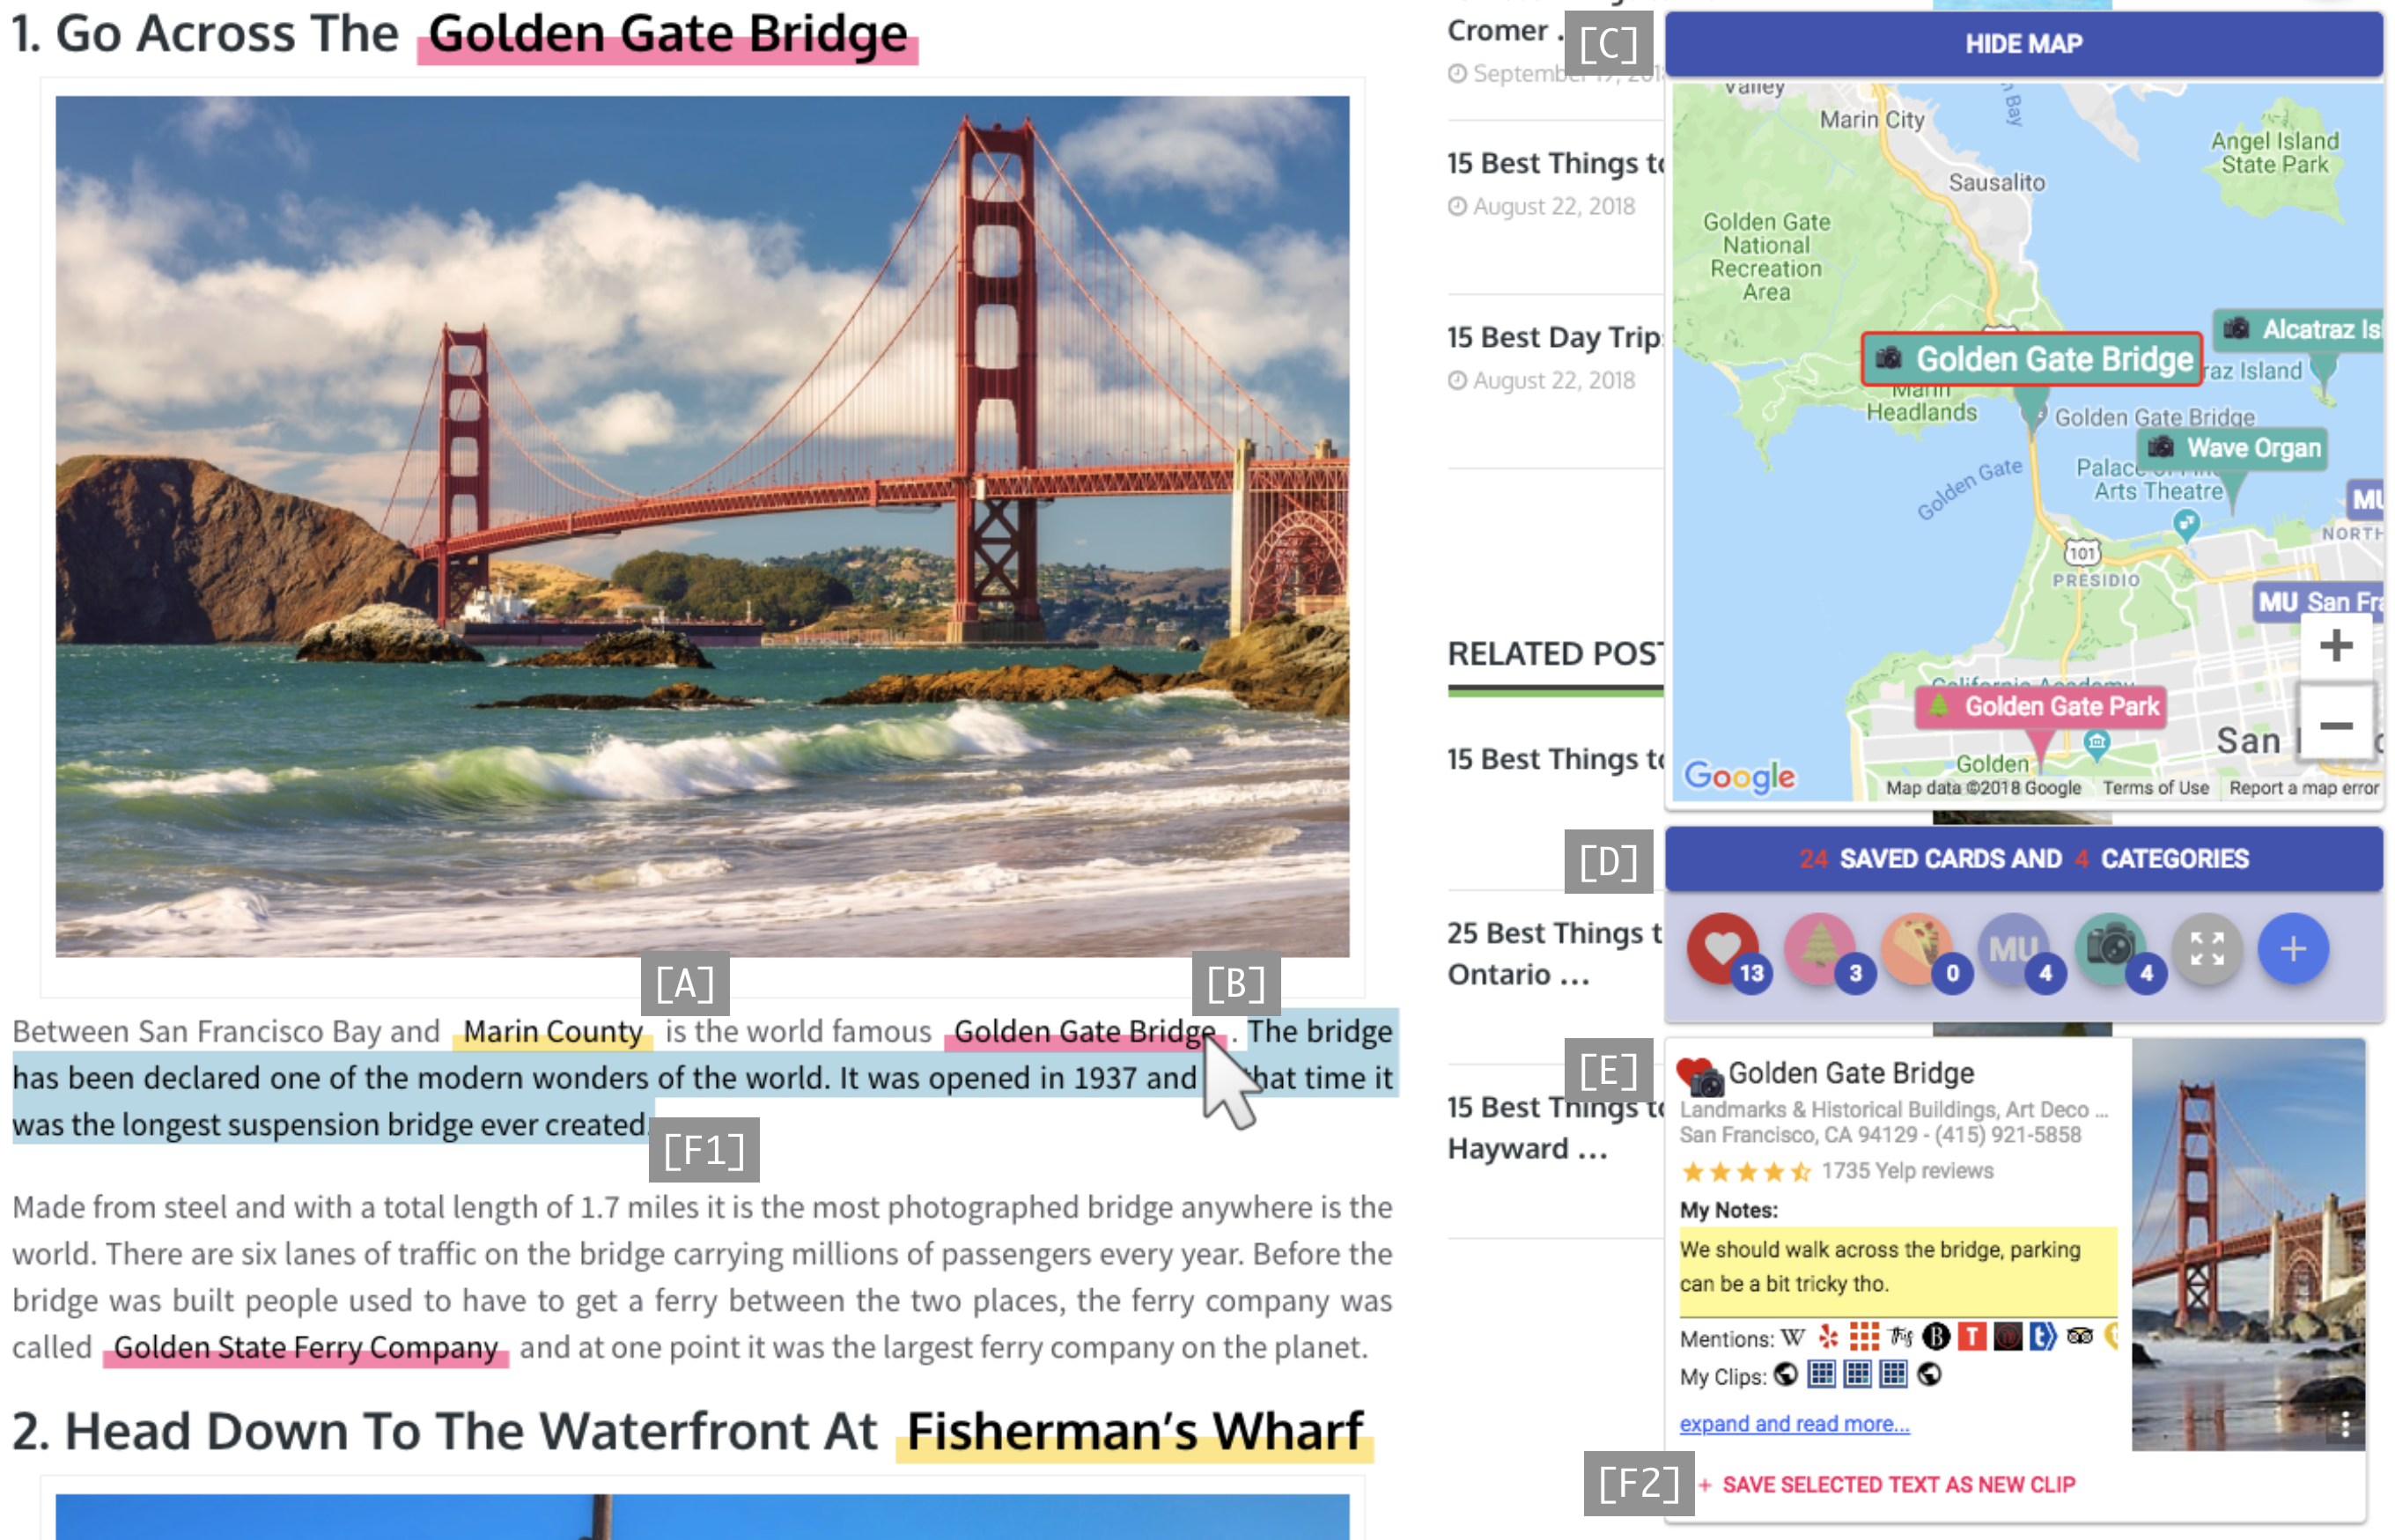
\includegraphics[width=1\textwidth]{Chapters/Weaver/main3.png}}
    \caption[An overview of the Weaver browser add-on.]{An overview of the Weaver browser add-on. Weaver identifies and highlights entity mentions on webpages [A,B] to indicate additional information is available. Highlights in red [B] indicates users had previously interact with the entity. Hovering an mention [B] brings out its corresponding entity card [E] as an overlay, with relevant information ``infused'' from other pages and knowledge bases as \emph{mentions}. Users can also save notes or selected sentences [F1] to a card as \emph{clips} [F2]. Saved clips are then automatically ``diffused'' to other webpages that mentioned the same entity. Users can also create categories [D] and drag the card under them. Finally, the Map view [C] shows its location in context of previously saved entities.}
    \label{fig:main_fusion}
\end{figure}

Whether planning a trip to a new city, figuring out which camera to purchase, or researching the different treatments for a medical issue, learning and searching for information online has become the most common way that people make sense of the world today \cite{mar2006exp,pirolli1999information}. People spend a significant amount of time exploring available options and gathering evidence about them that are scattered across multiple webpages in order to make informed decisions.  Estimates suggest that up to 33\% of the time spent online \cite{mar2006exp,kellar2007field,rose2004understanding}, or, as of 2009, around 24 billion hours per year in the US alone, are spent doing this type of aggregation and synthesis \cite{forrester}. 

We believe this problem of synthesizing information across sources is increasingly relevant as online information and misinformation (such as fake news and shill reviews) continues to expand. Past studies have shown users rely on aggregating from multiple sources in order to verify online information as credible and make decisions \cite{fox2000online,cotten2004characteristics,racherla2012perceived}, but the process can be ``tedious and cumbersome'' leading to ``opening several tabs ... and then manually switch[ing] between them while trying to remember information on different pages'' \cite{greis2017increasing}.  Anecdotal evidence for this can also be seen in the rise of aggregation-based sites such as Metacritic or Wirecutter, but such aggregators cannot cover all decision making scenarios nor able to take into account the personal context and goals of different users. In our own informal interviews on people's past experiences with trip planning and examining their notes, we also discovered similar needs and challenges -- they compared a large number of options based on evidence gathered from multiple sources, but struggled with managing large numbers of options and sources. 

In this paper, we focus on the domain of travel planning, because it has a number of characteristics that make it a good task to test new sensemaking and exploratory search approaches. For example, while it does not require a strong domain knowledge, useful information is often scattered across many sources; there is a strong degree of contextualization and personalization needed (e.g., traveling somewhere with kids is very different than without); and evidence such as reviews can be noisy and subjective \cite{zhang2012human,chen2015tripplanner}. Consider for example planning a trip to a new city: there may be hundreds of possible restaurants to dine at, attractions to see, and places to stay, each with corresponding evidence about its suitability for an individual's goals and preferences. Evidence about each of these options is often spread out across multiple search results, such as Yelp or TripAdvisor reviews, top ten lists, travel blogs, or forum posts. It can be a challenging process of intense cross-referencing and note taking to synthesize this evidence and to record how it meets a user's goals, with little scaffolding or intelligence built into the browser \cite{o1996towards,marshall1999introducing,tashman2011liquidtext,bianchi2015designing}.

%As the amount of user-generated content on the internet continues to grow, supporting users to benefit fully from large repositories of rich evidence is likely to become increasingly important \cite{mudambi2010research,gan2012helpfulness}.

%to To make an informed decision Cross-referencing evidence across these sites and In order to compare different options and make informed decisions, users need to cross-reference a large number of webpages to synthesize evidence about each potential option.  However, this process of intense cross-referencing and note taking can be disruptive when reading and consuming information \cite{o1996towards,marshall1999introducing,tashman2011liquidtext,bianchi2015designing}, and is poorly supported by current browser and note taking interfaces. As the amount of user-generated content on the internet grows, supporting users to benefit fully from large repositories of rich evidence is likely to become increasingly important \cite{mudambi2010research,gan2012helpfulness}.

Currently, such intelligence primarily takes the form of entity-centric approaches in search results interfaces \cite{guo2009named,lin2012active}. These approaches include showing entity cards with rich attributes for entity-bearing queries \cite{miliaraki2015selena,bota}, listing related entities as suggestions for subsequent queries (such as listing actors when searching about a movie) \cite{blanco2013entity,bordino2013penguins,klouche2015designing}, or extracting factual attributes about or relationships between entities (such as the director of a movie) \cite{balog2010overview,cheng2007entityrank,D15-1038}. While these approaches can efficiently provide factual and structured information about entities in search interfaces (such as when figuring out the location of a restaurant), they provide little support for the complex sensemaking situations described above, when there is no single objective answer that can be surfaced in a search results page (such as figuring out which city to visit for a vacation).

Instead of using entities as an answer or endpoint to a user's information needs at the query and retrieval stages, here we explore the idea that entities can also be useful during the reading and note taking stages by acting as the fabric connecting different information sources and use them to scaffold the user's mental model in complex exploratory search tasks. Leveraging entities has the potential to enable deeper and more fluid interactions with online information by focusing on meaningful concepts as the units of a user's externalized mental model rather than webpages. Furthermore, recent advances in entity linking algorithms have been particularly promising in bringing the ability to better understand web content to the browser where users read and learn from individual webpages \cite{spotlight}. For example, leveraging common entities mentioned across webpages to provide a sensemaking structure for users conducting complex exploratory searches and foraging across multiple webpages.

Specifically, in this paper, we explore a new paradigm for interacting with unstructured and subjective evidence about entities while reading and foraging from many webpages in exploratory search tasks. Since the user's personal evaluation of subjective information and how it meets their goal is critical in this situation, our design goal was to help the user to see scattered evidence about an entity in one place while also attaching personal notes and web clippings. These together serve as a way to build up an external mental model and track search progress.

To investigate our entity-centric approach, we developed a prototype browser add-on called Weaver. Weaver allows users to keep track of information scattered across multiple sources by ``infusing'' evidence about an entity from other information sources (webpages and knowledge bases) to the webpage the user is currently reading. It also ``diffuses'' users' thoughts about different entities across webpages where the same entities are mentioned for future reference and to accumulate more evidence. In our user study, we tested how participants utilized our entity-centric approaches while conducting a complex exploratory search task, focusing on whether Weaver allowed them to explore, gather, reuse, and accumulate evidence about entity options across multiple webpages. To control for task complexity, the primary domain on which we aimed to test Weaver was a pre-defined travel planning task (described in the Study Design section). With 24 participants and a baseline interface as a between subject condition, we found that participants using Weaver collected nearly 3 times more evidence across 60\% more pages while simultaneously being more selective in the options they explored. Furthermore, we describe qualitative evidence of the value in infusing of evidence from other webpages and diffusing users' notes across webpages. Finally, we discuss implications for the design of future intelligent interfaces that can better understand the information being consumed by their users by taking advantage of advances in natural language processing to support online sensemaking in various scenarios.




\section{Related Work}

\subsection{Sensemaking and the Web}

The importance of sensemaking and complex exploratory search on the web has been studied in depth by many researchers. Past work have identified a persistent challenge that valuable information for many topics is scattered across many different sources that are independent of one another and incur a high cost for bringing them together \cite{bhavnani2005difficult,mar2006exp,marshall1999introducing,kittur2013costs}. Theories of sensemaking suggest several cognitive tasks involved that could be supported through novel interactive tools, ranging from finding potentially relevant items, to triaging items based on reliability and relevance, to collecting evidence relevant to each item and organizing items into categories or structures \cite{russell1993cost, takayama2008tracing, hearst2013sewing}. We draw on these theories to select the set of cognitive tasks we are interested in supporting through entity-centric interaction approaches, which are typically complex and about synthesizing information, rather than simple fact-finding tasks \cite{mar2006exp, white2006supporting}.

\subsection{Recognizing Entities in Text}

Significant research has gone into entity-centric approaches for improving web search results pages due to the ubiquity of entities in online sensemaking. Researchers have found that entity-bearing and -category queries accounted for up to 85\% of web search traffic \cite{guo2009named,lin2012active}. This has led to significant academic and commercial efforts devoted to building large-scale entity databases (such as DBPedia \cite{dbpedia}, Yelp\footnote{http://yelp.com}, and Google Places\footnote{https://developers.google.com/places/web-service/intro}), and significant research on ways to identify entity mentions in plain text \cite{spotlight} and using them to enrich search interfaces. This involves both recognizing the same entity mentioned in different surface forms (e.g., MoMA and Museum of Modern Art) and resolving ambiguous surface forms to the right entity based on its surrounding text. Major threads of research that uses entities to improve search interfaces includes showing entity cards for entity-bearing queries \cite{bota,miliaraki2015selena}, answer factual questions  \cite{D15-1038}, and showing related entities as query suggestions \cite{blanco2013entity, bordino2013penguins,klouche2015designing}. We build on these recent advances in entity recognition and large-scale entity databases, but instead of focusing on the search interface and simple navigation we investigate the less-explored design space of supporting complex sensemaking across webpages opened in the browser through entity-aware interactions.


\subsection{Weaving Together Scattered Information across Sources}

Due to the scattered nature of information on the Web \cite{bhavnani2005difficult}, research has explored ways to connect relevant information distributed across different webpages. One set of top-down semantic web approaches involve incentivizing content publishers to provide machine readable annotations, such as using semantic web markups \cite{karger2004haystack, berners2001publishing,berners2001weaving}. However, such approaches have often failed to gain momentum due to issues such as a lack of available end-user tools that can consume these annotations \cite{whatwentwrong}. Alternatively, researchers have built bottom-up systems that exploit detecting entity mentions in articles, and used them as anchor points to connect to other information sources to enhance the reading experience. For example, Wikify identifies entity keywords in articles and creates hyperlinks to their Wikipedia entries for navigation \cite{mihalcea2007wikify}, and Experience-Infused
Browser links entity mentions in articles to past social interactions (such as emails) for making ``serendipitous connections'' \cite{hangal2012effective}.

Our approach is inspired by these bottom-up approaches in the context of recognizing entities mentioned in webpages opened in the browser. However, our work differs in several important ways: 1) instead of surfacing simple facts or links to articles or emails, we focus on providing context for people to understand complex information spaces; 2) we support the transition from viewing context to saving information; and 3) we propagate saved information to all other instances that entity is shown, allowing users to build up an entity-based mental model of the space.

%Instead of navigating users to a separate page, we used an in situ design that allowed users to hover over an entity mention to bring out its entity card \emph{infused} with relevant information extracted from other information sources. In addition to information from external knowledge sources (such as Wikipedia), we also used the entity cards to show relevant information extracted from other opened webpages that also mentioedn the same entity for lightweight cross-referencing.


\subsection{Note Taking and Saving Information Online}

Collecting information online during complex sensemaking tasks can be costly for the users, requiring them to cross-reference between pages and their notes in order to gather all the evidence. This frequent context switching between different documents and taking notes can be distracting, and even prohibitive for users to investigate deeper or to take notes in order to avoid disrupting the flow of reading \cite{o1996towards,marshall1999introducing,tashman2011liquidtext,bianchi2015designing}.

On one end of the spectrum, research has focused on allowing users to extract and save structured information from webpages more efficiently from a single document using end-user programming \cite{thresher,huynh2005piggy,dontcheva2006collecting,dontcheva2007relations} and interaction techniques \cite{bier2006entity,stylos2004citrine}. Our work is motivated by these studies highlighting users' desire to collect information about entities, but instead of focusing on structured and objective attributes we are interested in additionally gathering descriptive and subjective evidence, such as how a restaurant is described in a top ten list. Furthermore, many of the approaches above define patterns for extracting multiple entities from a single page, whereas we are more interested in finding evidence related to entities across multiple pages where the structure of those pages might differ significantly.

On the other end of the spectrum, researchers have also explored using in situ interfaces, such as sidebars or on page annotations, to reduce the costs of switching between reading and note taking and collecting from multiple information sources \cite{romat2019spaceink,tashman2011liquidtext,notetoself,van2011finders,schraefel2002hunter}. Our work is also situated in this thread of research on reducing the costs of switching and sensemaking. However, instead of persisting notes on individual documents, our approach persists notes on individual entities which may then appear across multiple documents. 

%Unstructured note taking approaches also run into challenges with scaling for reusing and organizing large collections of saved notes.  For example, a prior system, NoteToSelf, reported that their participants relied on skimming or targeted search using keywords from memory for re-finding previously saved notes, which led to a large portion of user notes rarely re-accessed nor deleted \cite{notetoself}. Fundamentally, note taking software treats options mentioned on webpages and users' notes about them as independent, and cross-referencing between webpages and their notes to accumulate evidence for the same options can be incur high costs. In this work we explore an entity-centric approach that connects different webpages and users' notes through common entity mentions, allowing us to automatically resurface previously saved notes as they became relevant to users' current reading.




\begin{figure}
    \centering
    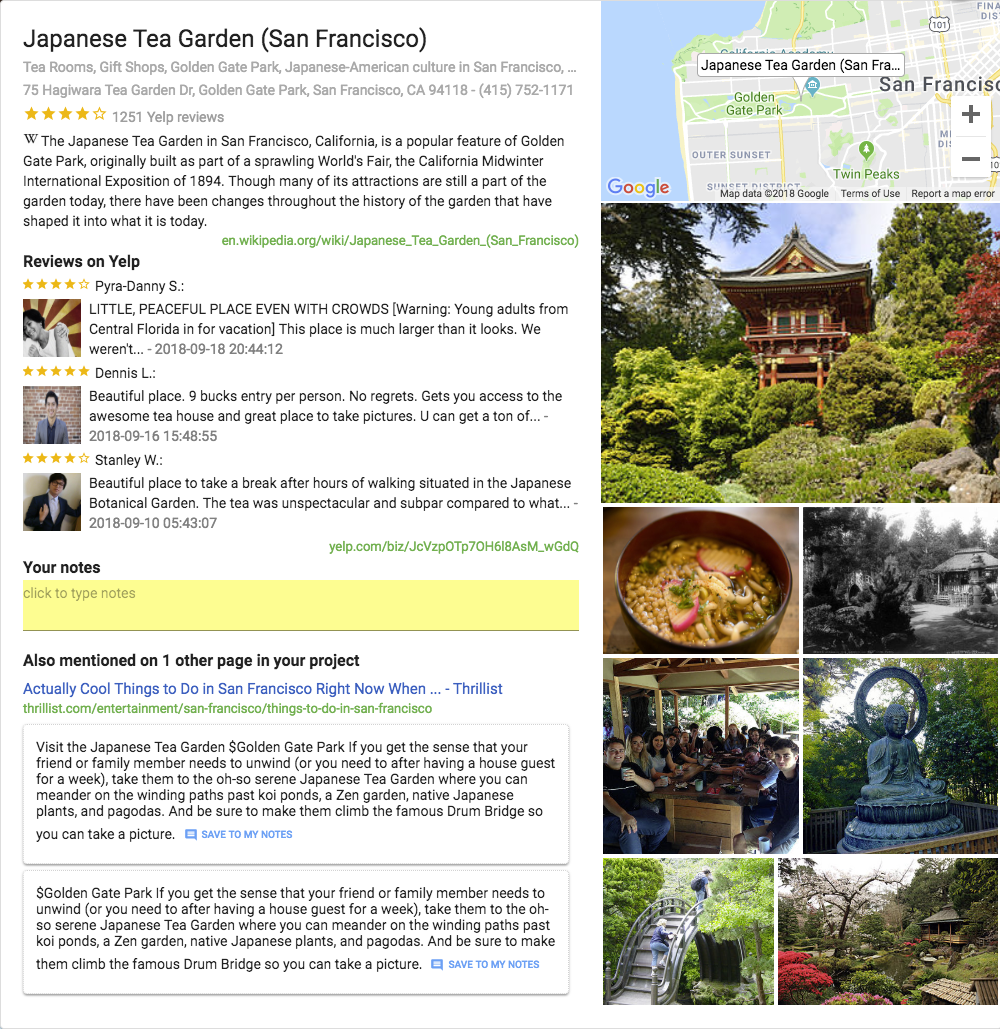
\includegraphics[width=1.0\columnwidth]{Chapters/Weaver/expanded.png}
    \caption[Expanded view for an entity card.]{Expanded view for an entity card showing information \emph{infused} from external knowledge sources (Yelp and Wikipedia), user's notes, and evidence of the same entity from other webpages in the exploratory search task. See Figure~\ref{fig:main_fusion} for the non-expanded view of an entity card.}
    \label{fig:expanded_fusion}
\end{figure}


\section{System Design}

We introduce Weaver, a novel browser add-on that uses an entity-centric approach to facilitate sensemaking across webpages in exploratory search tasks. 
Unlike previous approaches that focused on either enriching search results pages \cite{syed2017optimizing,miliaraki2015selena}, saving information from individual documents \cite{tashman2011liquidtext,thresher}, or providing separate note taking interfaces \cite{dontcheva2007relations}, we focused on supporting sensemaking across multiple information sources by weaving them together through common entity mentions. This allows users to both evaluate potential options with more context and re-access previously saved information about an option with lowered effort.
Figure \ref{fig:main_fusion} shows an overview of how an exploratory searcher planning a trip might use Weaver. Weaver provides users a lightweight overlay interface embedded on and synced across webpages opened in different browser tabs, allowing users to make quick and lightweight cross-referencing without switching between tabs, windows, or applications.

The two core components of Weaver scaffold sensemaking through entities in two primary ways, which we introduce as ``\emph{Infusion}'' and ``\emph{Diffusion}.'' First, when users open a webpage from their search results, the system ``infuses'' the webpage with relevant snippets about mentioned entities from other webpages in their search results and external knowledge sources to help users cross-reference and evaluate newly encountered options. Second, when users save notes or extract content from a webpage, the system ``diffuses'' them to mentions of the same entities in other webpages of the same task, allowing them to easily access previously saved information without having to switch to and search through their notes a separate interface. In the next subsections, we will first describe in detail both Infusion- and Diffusion-based features, a project overview interface, and finally describe how entities were automatically identified and linked to external knowledge bases.

\subsection{Infusion: Gathering Evidence from other Webpages}

One significant challenge in making sense of a given topic on the internet is that relevant information is scattered across multiple places, and it is difficult to find those places and to synthesize what they say. Doing so is valuable in understanding the popularity and prevalence of a given option (e.g., how often a restaurant is mentioned in lists of top restaurants, what are the various lists of top restaurants) as well as the context and potential biases in how it is described (e.g., is it suitable for a date night, are the pages it is mentioned on reliable). Instead of using them at only the beginning on search results pages, entities could provide a scaffold for improved in situ interactions throughout the browsing process to help users more quickly get a sense of the popularity and context of different options without going to all the different pages on which they are mentioned, as well as providing ``pivot points'' to see what other sources mention an option.

For example, in Weaver, a user planning a trip to a new city can open an article from a travel blog and see all the destination and restaurant mentions highlighted in yellow. Hovering on a attraction surfaces contextual snippets from other webpages that also mention that attraction, so the user can understand its relevance to their own goals without interrupting their flow of reading (Figure~\ref{fig:main_fusion}, B and E). Other sources of information can be brought in and surfaced at the same time, such as Yelp review scores and Wikipedia descriptions. By infusing this information using the entity as a pivot, it is possible that users could both reduce the number of items they need to keep track of (by filtering out non-matching items earlier) and better understand the context of the items they do keep. Meanwhile, the number of sources that mention the item provides implicit feedback as to its popularity within the searches the user has made; their URLs may provide context as to the reliability of those sources; and they may provide additional sources for finding information about other restaurants if they mention a restaurant the user knows they like. 

%A common activity in complex exploratory search involves collecting information from multiple sources and make informed decisions.
%Our preliminary survey, as described in the Introduction, showed that 88\% of participants ``use information from multiple webpages to verify uncertain information.'' % removed from intro
%echoed by our preliminary study described in the Introduction in which 88\% of participants reported that they typically gather evidence from multiple sources ``in order to verify uncertain information.'' %Similarly, 83\% reported that they would typically perform at least 4 searches to gather information when planning a trip, and 50\% would spent at least 4 hours searching when purchasing something important or expensive.
Weaver supports this need by ``infusing'' entities mentioned on a page with context pulled from other webpages mentioning the same entity or entries in external knowledge sources (in our current implementation, DBpedia and Yelp). When users open a webpage, entity mentions that were recognized by Weaver are highlighted with a half-height yellow highlight (Figure \ref{fig:main_fusion}, A) to indicate they have information from other sources. By hovering over an entity, a user can see an ``entity card'' (Figure \ref{fig:main_fusion}, E) which displays those sources and relevant information (e.g., number of stars on Yelp, paragraphs from other websites in which the entity was mentioned) which a user can use to gain context about the entity beyond the current webpage \cite{bota}. To read the mentions, the user can click on the icon of each external source to see an extracted snippet. Alternatively, the user can also expand the Card to see a larger view (Figure~\ref{fig:expanded_fusion}), showing all mentions, multiple images, and a map of the location using metadata from Yelp and/or DBpedia. 

%As a running example, a user planning a trip to a new city might open an article from a travel blog and see all the destination and restaurant mentions highlighted in yellow by Weaver. As the user reads the article, he or she finds a highlighted restaurant and the author recommended it for reasons that also fit our user's personal interests. However, instead of relying on this single piece of evidence, the user hovers over the restaurant name to query for its entity card for additional information. The entity card contains Yelp review scores, Wikipedia description, and a list of relevant snippets from other webpages from the user's previous searches. After reviewing these information, the user drags the entity card under the restaurant category created previously. 

\begin{figure}
    \centering
    \frame{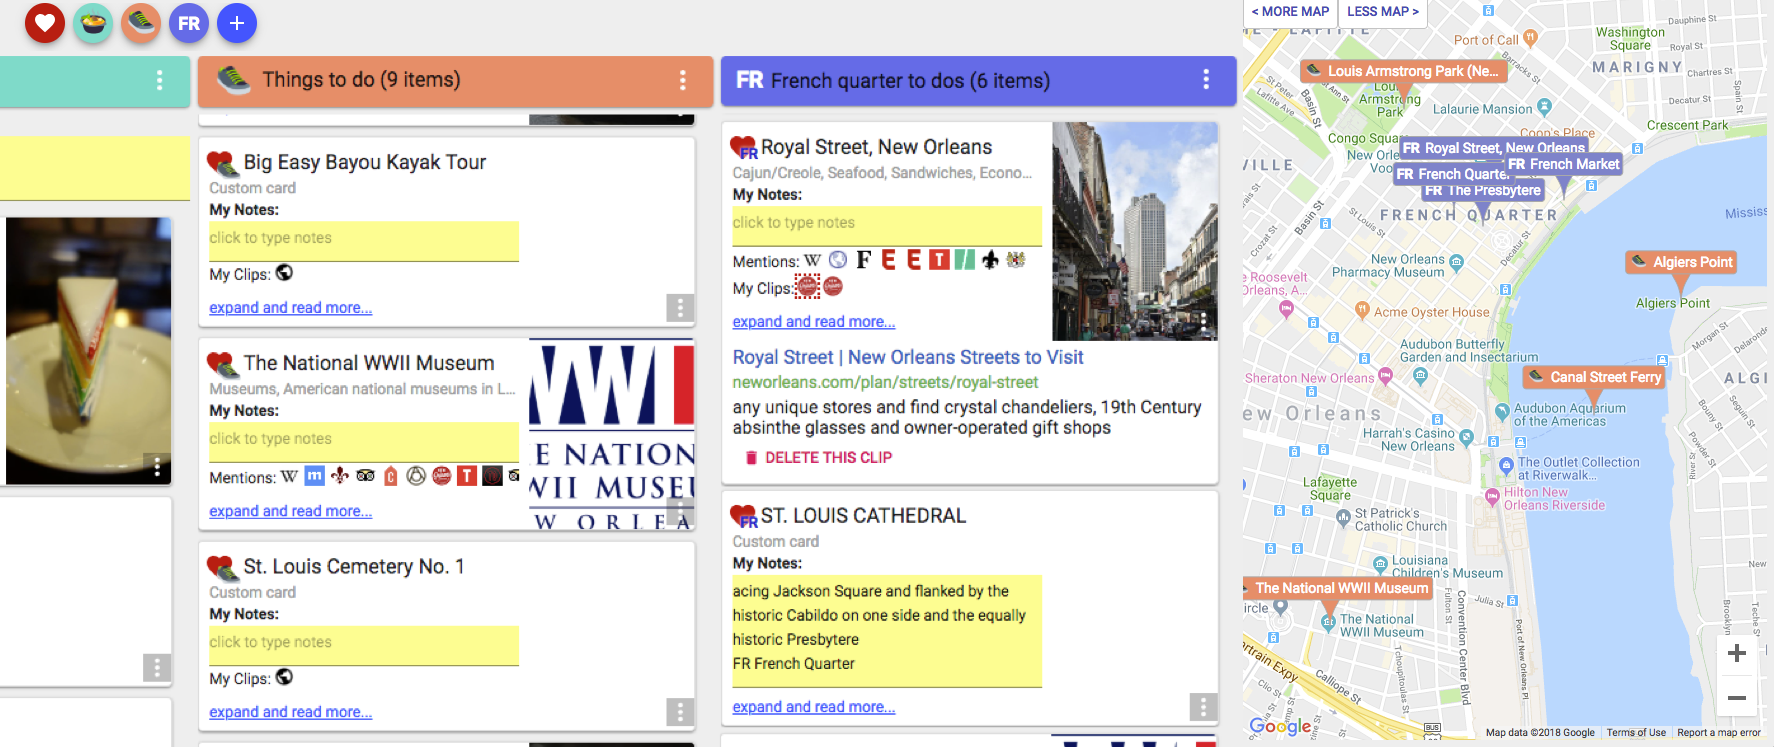
\includegraphics[width=1\textwidth]{Chapters/Weaver/project2.png}}
    \caption[An project overview page created by one participant.]{An project overview page created by one participant after searching for 50 minutes, containing entities saved under different categories, text clips from multiple webpages, and typed notes. Custom cards were created, including one for a kayaking tour that was not available on Yelp and DBpedia. The entity cards were scaled for clarity in this figure.}
    \label{fig:project_fusion}
\end{figure}





\subsection{Diffusion: Propagating Notes to other Webpages}

After using ``infused'' context to judge the relevance and suitability of options (i.e., entities), users often need to keep track of and organize the options they found valuable. At the same time, users may evaluate newly encountered options against ones they have already saved. Typically, this happens by copy-pasting or typing entity names and notes into a separate interface, for example a separate document or email or note taking software (e.g., Evernote). Researchers have tried to lower the switching cost involved in this interaction \cite{o1996towards,tashman2011liquidtext}, for example, by adding a sidebar to the browser for taking free-form notes \cite{notetoself}. However, in the cases when the user encounters additional evidence about an option they already have information about, they need to re-find it in the external system before being able to continue. This high interaction cost can be prohibitive as it lead to disruptions of user's flow of reading \cite{chang2016supporting,tashman2011liquidtext,o1996towards,marshall1999introducing}.

Weaver addresses this challenge by ``diffusing'' notes that users associate with an entity to all other webpages in the project that also mentioned the same entity, reducing the need for user-driven re-finding. Continuing with our running example of trip planning from the previous subsection, imagine that after the user reviews the information in a restaurant entity card, he or she decides to take notes and save the restaurant for future reference. To do so, the user can add various levels of annotation to the card, including just ``hearting'' it to save it in the Saved Cards view as uncategorized  (Figure \ref{fig:main_fusion}, top-left corner of E), typing notes about reasons for saving it (Figure \ref{fig:main_fusion}, yellow region in E), or selecting sentences (Figure \ref{fig:main_fusion}, around B) from the webpage to add to the entity card as a clip (Figure \ref{fig:main_fusion}, E). When the user moves on to other webpages in the project, mentions of the same restaurant will be highlighted in half-height light red (Figure \ref{fig:main_fusion}, B), indicating that the user previously interacted with this entity, and upon hovering will see its entity card with annotations and clips they have previously added. 


Using this entity-centric approach, users can save notes of information collected across webpages under entity cards without having to switch back and forth between the browser and note-taking software, and easily re-find and reuse previously saved information when encountering the same entities on other webpages. To recover from cases where an entity of interest was not recognized by Weaver automatically, users can manually create entity cards using interactions as described in the next subsections.



\subsection{Project Overview and Organizing Entities}



As users in exploratory search tasks gradually progress from discovering entities and gathering evidence to focus more on synthesizing and making decisions, they may also need to organize and compare the collected entities. For example, in a travel planning task, users may want to group their entities into categories of restaurants, attractions, and hotels for comparison, and also to figure out the location and distances between the different entities to plan their trips.

In Weaver, in addition to simply ``hearting'' an entity card, users can also create categories with custom names, colors, and icons in the Saved Cards view (Figure \ref{fig:main_fusion}, D). To categorize an entity card, simply drag and drop it between categories. This allows users to start structuring any time during their exploratory search process when the need arises. Saved geographic entities (entities with coordinates metadata from Yelp and/or DBpedia) will also show up in the Map View  (Figure \ref{fig:main_fusion}, C) with their icons and color coded pins. In addition, when users hover over an unsaved geographic entity on the current webpage, its location is also shown on the Map view. This allows users to better situate a newly encountered option with previously discovered entities to make informed decisions. For example, a user could quickly figure out that a hotel recommendation on the current webpage is not relevant by noticing in the Map view that it is too far away from most attractions that they have saved previously from other webpages. At later stages of the exploration process, users might shift their focus from reading and gathering information to synthesizing and organizing information. For this, they can open the Project Overview page by clicking on the expand button in the Saved Cards view to see all their entity cards listed in multiple columns of each category along with an integrated map view (Figure \ref{fig:project_fusion}).

\begin{figure}
    \centering
    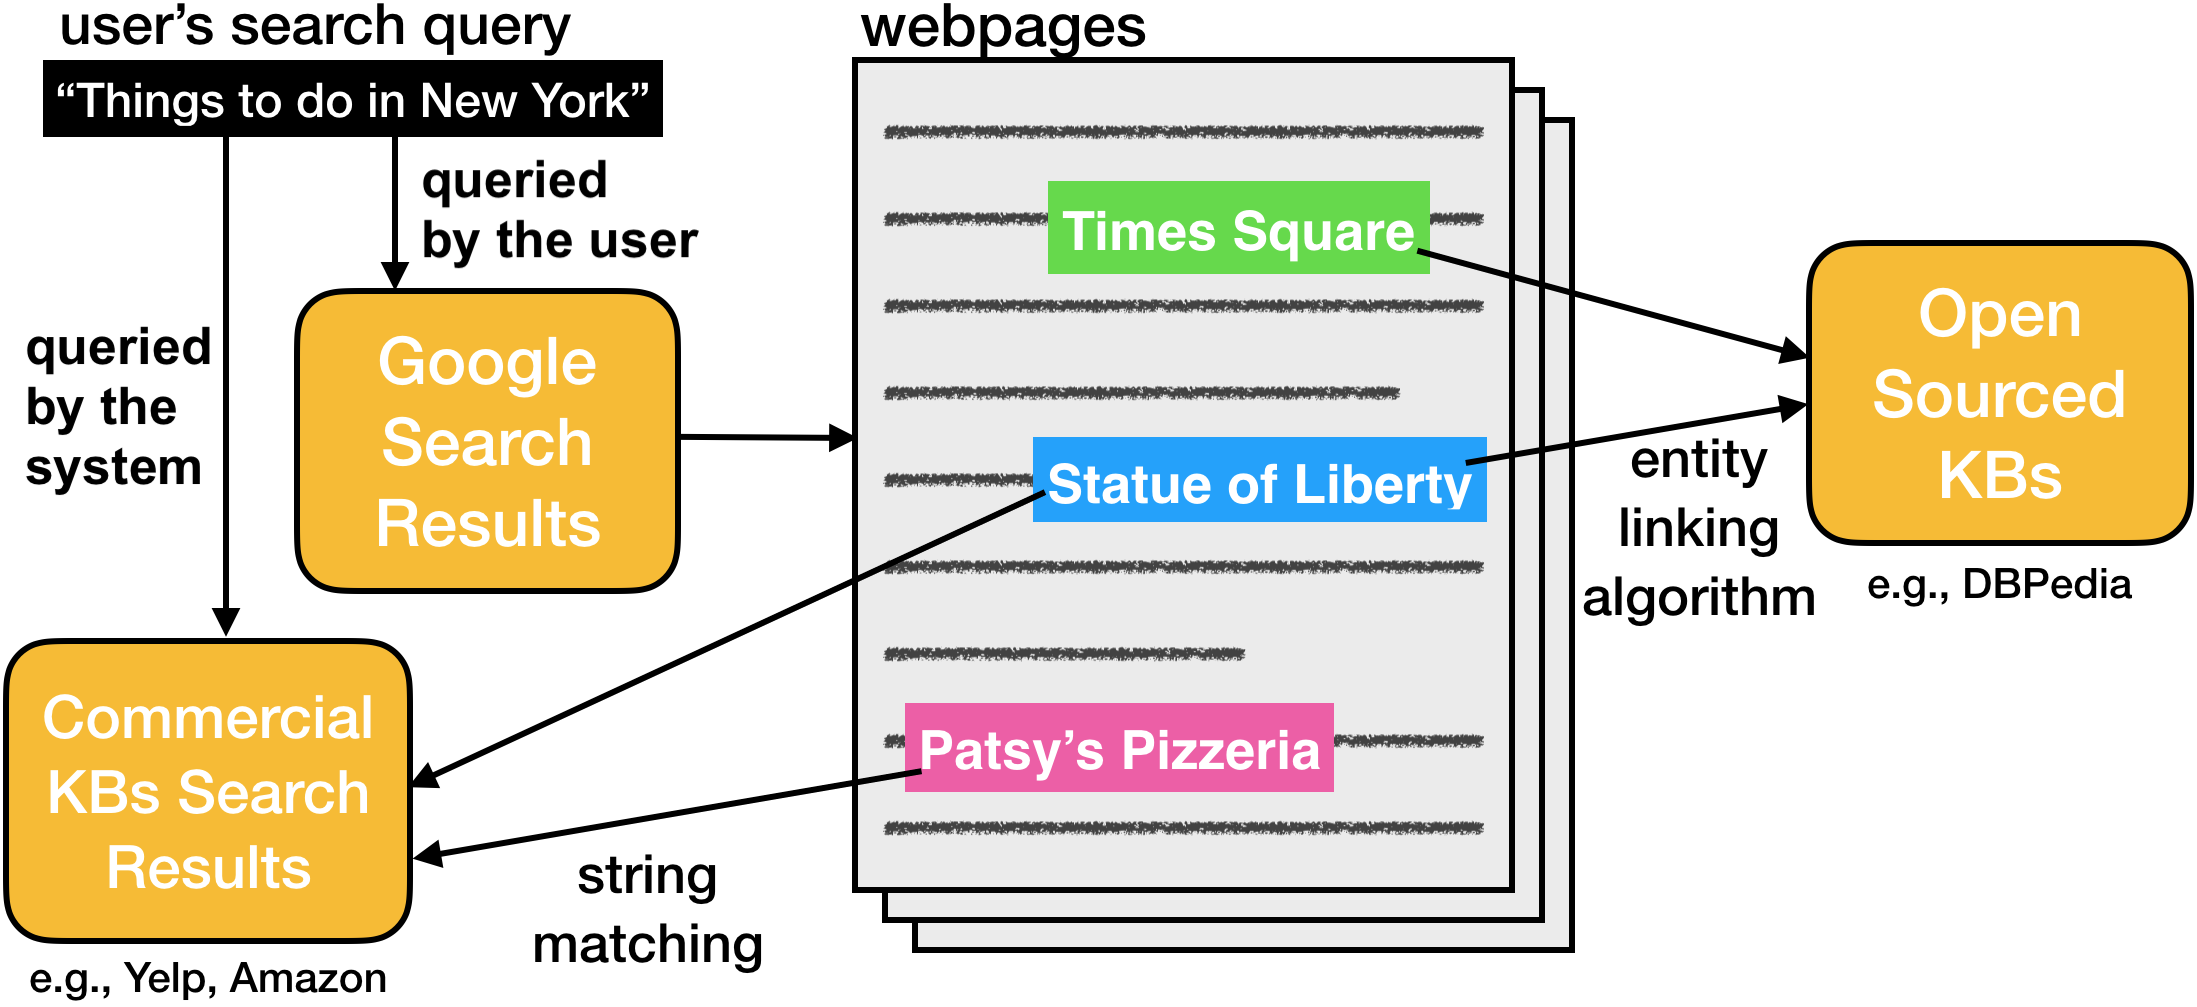
\includegraphics[width=0.5\columnwidth]{Chapters/Weaver/entity_linking2.png}
    \caption[Linking entities from webpages to open and commercial knowledge bases.]{Weaver links entity mentions from webpages to both open and commercial knowledge bases.}
    \label{fig:entity_linking_fusion}
\end{figure}

\subsection{Linking to Open and Commercial Knowledge Bases}

To drive these operations and connect the different webpages, Weaver uses the DBpedia Spotlight algorithm \cite{spotlight} to automatically identify common entities mentioned in the different webpages. In our implementation, we use Yelp and DBpedia as our entity repositories and focus on travel planning tasks, but other knowledge bases can also be used or added to support other types of projects. For example, using the Microsoft Academic Graph\footnote{https://www.microsoft.com/en-us/research/project/microsoft-academic-graph/} and the Gene Ontology \cite{gene} as knowledge bases to support literature review projects in biology.

As users search on Google, Weaver parses the HTML of the search results pages to obtain the list of webpages. In the background, Weaver analyzes the content of webpages to identify entities mentioned using the following methods (Figure~\ref{fig:entity_linking_fusion}). First, it uses the Spotlight library \cite{spotlight} to identify entities mentioned in different surface forms (e.g., ``San Francisco Museum of Modern Art'' and ``SFMoMA'') to DBpedia which contain rich attributes extracted from Wikipedia. Unlike DBpedia, Yelp is a commercial services in which neither the entity database nor a pre-trained entity linking model were publically available. In order to identify Yelp entities in webpages, we use keywords and a location extracted from the original query term users performed on Google (e.g., ``best sushi bars in new york'') to query the Yelp Search API\footnote{https://www.yelp.com/Fusion} for a list of 450 related Yelp entities. This allows Weaver to retrieve from closed databases for entities that match with users query intent and information needs. Simple string matching is used to identify mentions of any Yelp entities on each webpage.

To avoid showing duplicate entities from DBpedia and Yelp and to improve the coverage of identifying Yelp entities, Weaver use a location-based heuristic to merge entities from the two sources: two entities are merged if 1) they are from different knowledge bases, 2) have overlapping surface forms listed in the knowledge bases, and 3) have geographic coordinates that are less than two kilometers from each other. Using simple string matching to identify Yelp entities on webpages can have limited coverage since Yelp only lists one surface form for each entity (e.g., the name of a restaurant). However, if a Yelp entity was merged with a DBpedia entity, it is automatically applied to mentions of different surface forms as identified by the entity linking algorithm \cite{spotlight}. For example, once the Yelp entity ``San Francisco Museum of Modern Art'' was merged with its corresponding DBPedia entity, information from Yelp is automatically linked to its mentions in different surface forms listed in DBPedia, such as ``SFMoMA''.
Finally, Weaver extracts the paragraphs around entity mentions from each webpage as supporting evidence along with the following structured data from the knowledge bases (Figure~\ref{fig:expanded_fusion}): location on a map, phone number, Yelp and Wikipedia categories, images, short descriptions from Wikipedia, average review scores and number of reviews on Yelp, and 3 Yelp reviews.


\begin{figure}
    \centering
    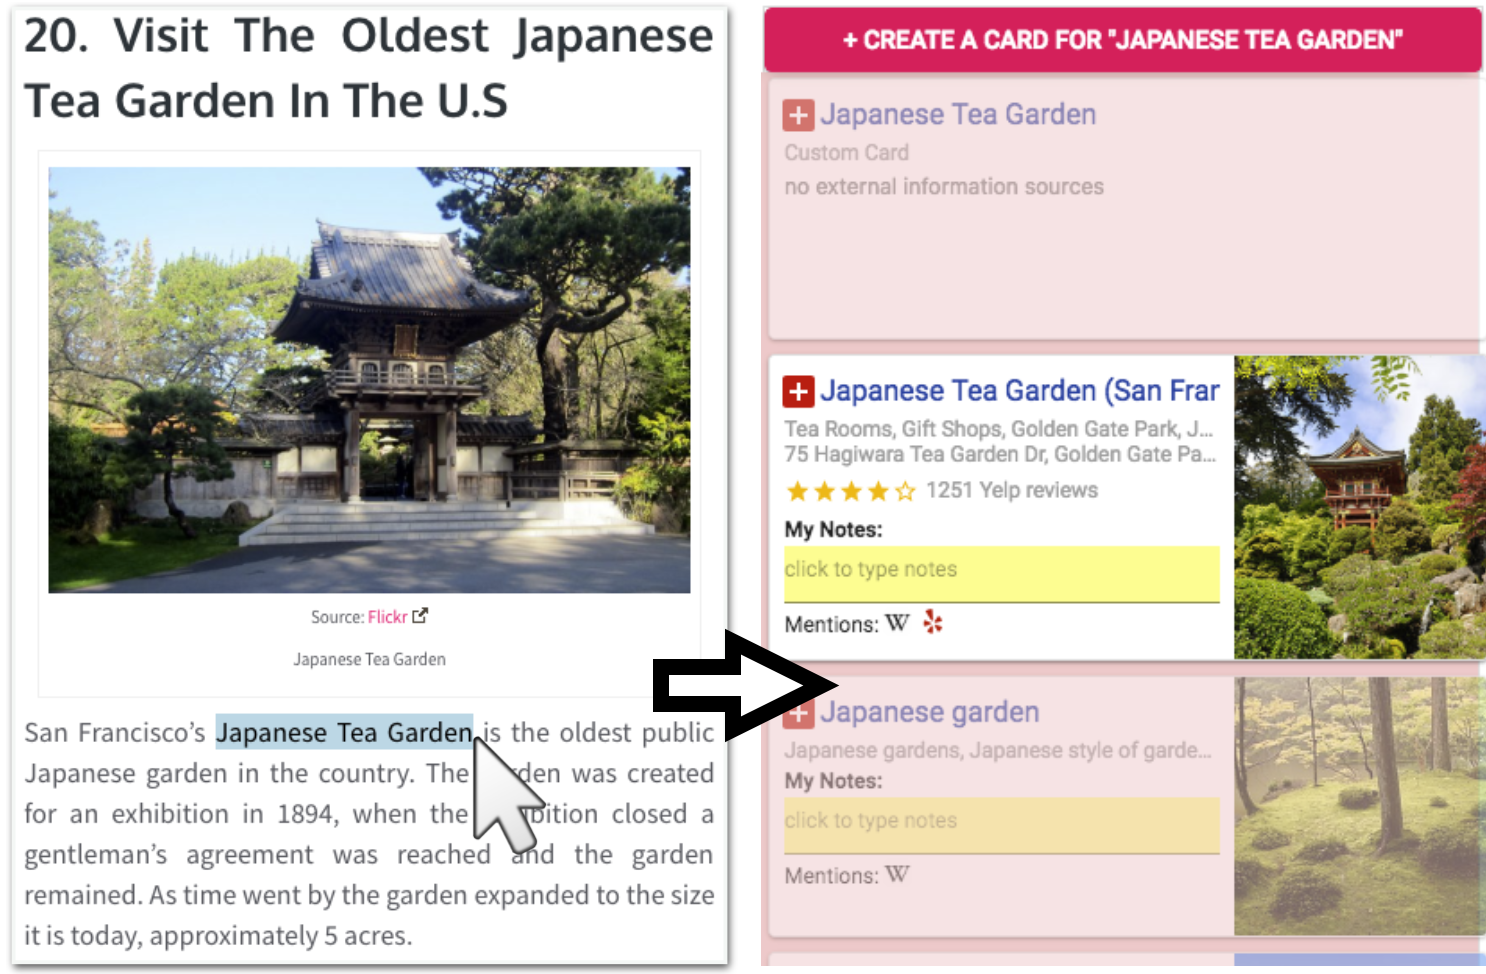
\includegraphics[width=0.5\columnwidth]{Chapters/Weaver/custom4.png}
    \caption[Creating manual entity cards.]{To create a missing entity, users can select a phrase (here, Japanese Tea Garden) on the page and see a list of candidates to choose from. In this case, the top 3 candidates were 1) a Custom Card not linked to external knowledge bases, 2) an entity card linked to a specific Japanese garden on both Yelp and DBpedia, and 3) and entity card linked to the general entity for Japanese gardens in DBpedia.}
    \label{fig:custom_fusion}
\end{figure}

While the state of entity recognition is continuously improving, a caveat of driving end-user interfaces with machine learning is potentially having the model make occasional mistakes that can degrade the user experience, and it is crucial to provide mechanisms for the users to recover from them \cite{lewis1995designing,lee2010gracefully,kocielnik2019will}. For example, in a trip planning task, a webpage might miss a popular destination not recognized by the Spotlight algorithm, not listed on DBpedia, or not covered in the top 450 results returned from the Yelp API.
To recover from cases where an entity of interest was not recognized by Weaver, the user can still create a custom entity card by first selecting the entity name on the webpage, and click on the ``Create Card'' button in Weaver (Figure \ref{fig:custom_fusion}). In the background, Weaver queries the two knowledge sources for candidates, merges the two results lists using the location-based heuristics described previously, and finally presents the list of candidates from which the user can pick.  Alternatively, if the entity was not found in the knowledge bases, the user can still create a custom entity card with no external entity information (Figure \ref{fig:custom_fusion}).
%In early pilot testing, we found a common user need for this in creating an ``ad hoc'' entity where there might not be a specific, concrete location or entity (e.g., creating a card to collect tips about packing for Machu Pichu or general descriptions of beaches in New England).
If a user created an entity card that was linked to DBpedia and/or Yelp entities, all the information that was associated with them will also appear on the user-created entity card. This ensures that users can still save and retrieve information to accumulate what they have learned, even when an entity mention was not automatically recognized by Weaver.

During development, we tested this algorithm on the top 10 Google search results for the query ``Things to do in new orlean''. The average time to analyze each webpage was 1.8s ($\sigma$=1.3s, max 4.3s, ran in parallel). The on-page highlighting of entities utilized MarkJS library\footnote{https://markjs.io/} which has a speed comparable to the in-page search feature of Chrome.% None of the participants in our study reported issues with performance.





%In addition, since Weaver depends on users' original search terms to obtain relevant entities via the Yelp Search API, webpages opened by typing URLs into the address bar does not support recognizing Yelp entities automatically in the current implementation. These issues may disrupt users' exploration processes, forcing users to resort to external tools for capturing information.
 
% To provide a way to recover from these situations, Weaver allows users to manually mark phrases on the webpage as entities and link them to entities in DBpedia and/or Yelp (Figure \ref{fig:custom}, we will describe in detail in the next subsection.)


\section{Evaluation}

\subsection{Study Design}


The main goal was to explore the benefits and challenges of our entity-centric approach, and how it affected the process of reading, cross-referencing, and collecting information during complex exploratory search tasks.
For this, we built a baseline system that also had an in situ interface, but with no on-page entity recognition support nor provided entity cards with rich information and as a structure for saving evidence. Similar to a prior system introduced in \cite{notetoself}, the baseline system consisted of a sidebar that can be opened on any browser tabs for note taking. However, instead of allowing participants to create itemized lists of short notes, our implementation allowed participants to type notes and/or copy and paste information into a large text input field (Figure~\ref{fig:baseline_fusion}). As participants typed or pasted information into the sidebar, it is automatically saved and synced across browser tabs in real-time where the sidebar was opened similar to online text editors, such as Google Docs, that are commonly used to supporting online research.

We are aware that Evernote web clipper and Google Doc are common tools based on our informal interviews, but we believed our in-situ baseline to be a stronger baseline for what we set out to measure -- whether the Infusion and Diffusion mechanisms can promote gathering and sensemaking across multiple sources: 1) Infusion and Diffusion benefits users when both collecting and organizing information, the Evernote clipper only supports collecting and would require significant effort for organizing --  it creates a new document for every clip, and requires managing and merging multiple documents in a separate interface to organize them. 2) On the other hand, we think our in-situ baseline closely resembles using a separate plain text document, and the in-situ design lowers the cost of collecting by removing the need to switch between application windows. Further, using a separate document as baseline would introduce an additional variable between the two conditions (in-situ vs separate UIs) when the in-situ design is not part of our core contribution

A lab study was conducted with 24 participants recruited from a local participant pool. The participants ranged from the age of 18 to 43 ($\bar{x}$=25.38, $\sigma$=5.53), 63\% were female, 33\% of were college students, and 38\% had a bachelor's degree. 
To control for task complexity, we used a predefined task to compare Weaver with the baseline system as a between subject condition with each system assigned to 12 randomly selected participants. The study began with a pre-survey for demographic information, followed by 50 minutes of exploratory search for the given task (described below). Finally, participants answered a post-survey and were interviewed about their experiences. During the study, we recorded the actions participants performed interacting with the two systems via either event logging (Weaver) or screen recording (baseline) for post-analysis. Each participant was compensated 15 USD.

The main task of travel planning was designed to test Weaver's ability to support collecting evidence from multiple sources to support decision making between many options and had the following instructions:

    \begin{tightquote}
You and your friends are going on a trip to New Orleans. Help the group figure out which places you should go and where to eat during the trip. 
    \end{tightquote}
    
\noindent We also used the following description as a motivator to encourage the participants to put in more research effort, derived from previous studies of sensemaking:

\begin{tightquote}
Imagine after this task you will share you found with your friend(s), along with a short summarization in an email. To convince your friend(s) of your choices, provide enough reasons and information about your choices.
\end{tightquote}
    
%\noindent Travel planning has a number of characteristics that make it a good task to test new sensemaking and exploratory search approaches. For example, while it does not require a strong domain knowledge, but information is often scattered across many sources; there is a strong degree of contextualization and personalization needed (e.g., traveling somewhere with kids is very different than without); and evidence such as reviews can be noisy and subjective \cite{zhang2012human,chen2015tripplanner}.  This domain also worked well with the backing knowledge bases in our implementation -- Yelp provided entities for local restaurants and tourist attractions with images and reviews, while DBpedia provided general entities extracted from Wikipedia.


%In addition to our primary domain, in a follow up study we recruited another 8 participants who used Weaver to conduct the following camera shopping task:



%\noindent After conducting the main task for 50 minutes, participants spent another 30 minutes answering a post-survey using both Likert-scale ratings and free-form responses focused on their experiences during the main task and to compare Weaver with their current practices.

\begin{figure}
    \centering
    \frame{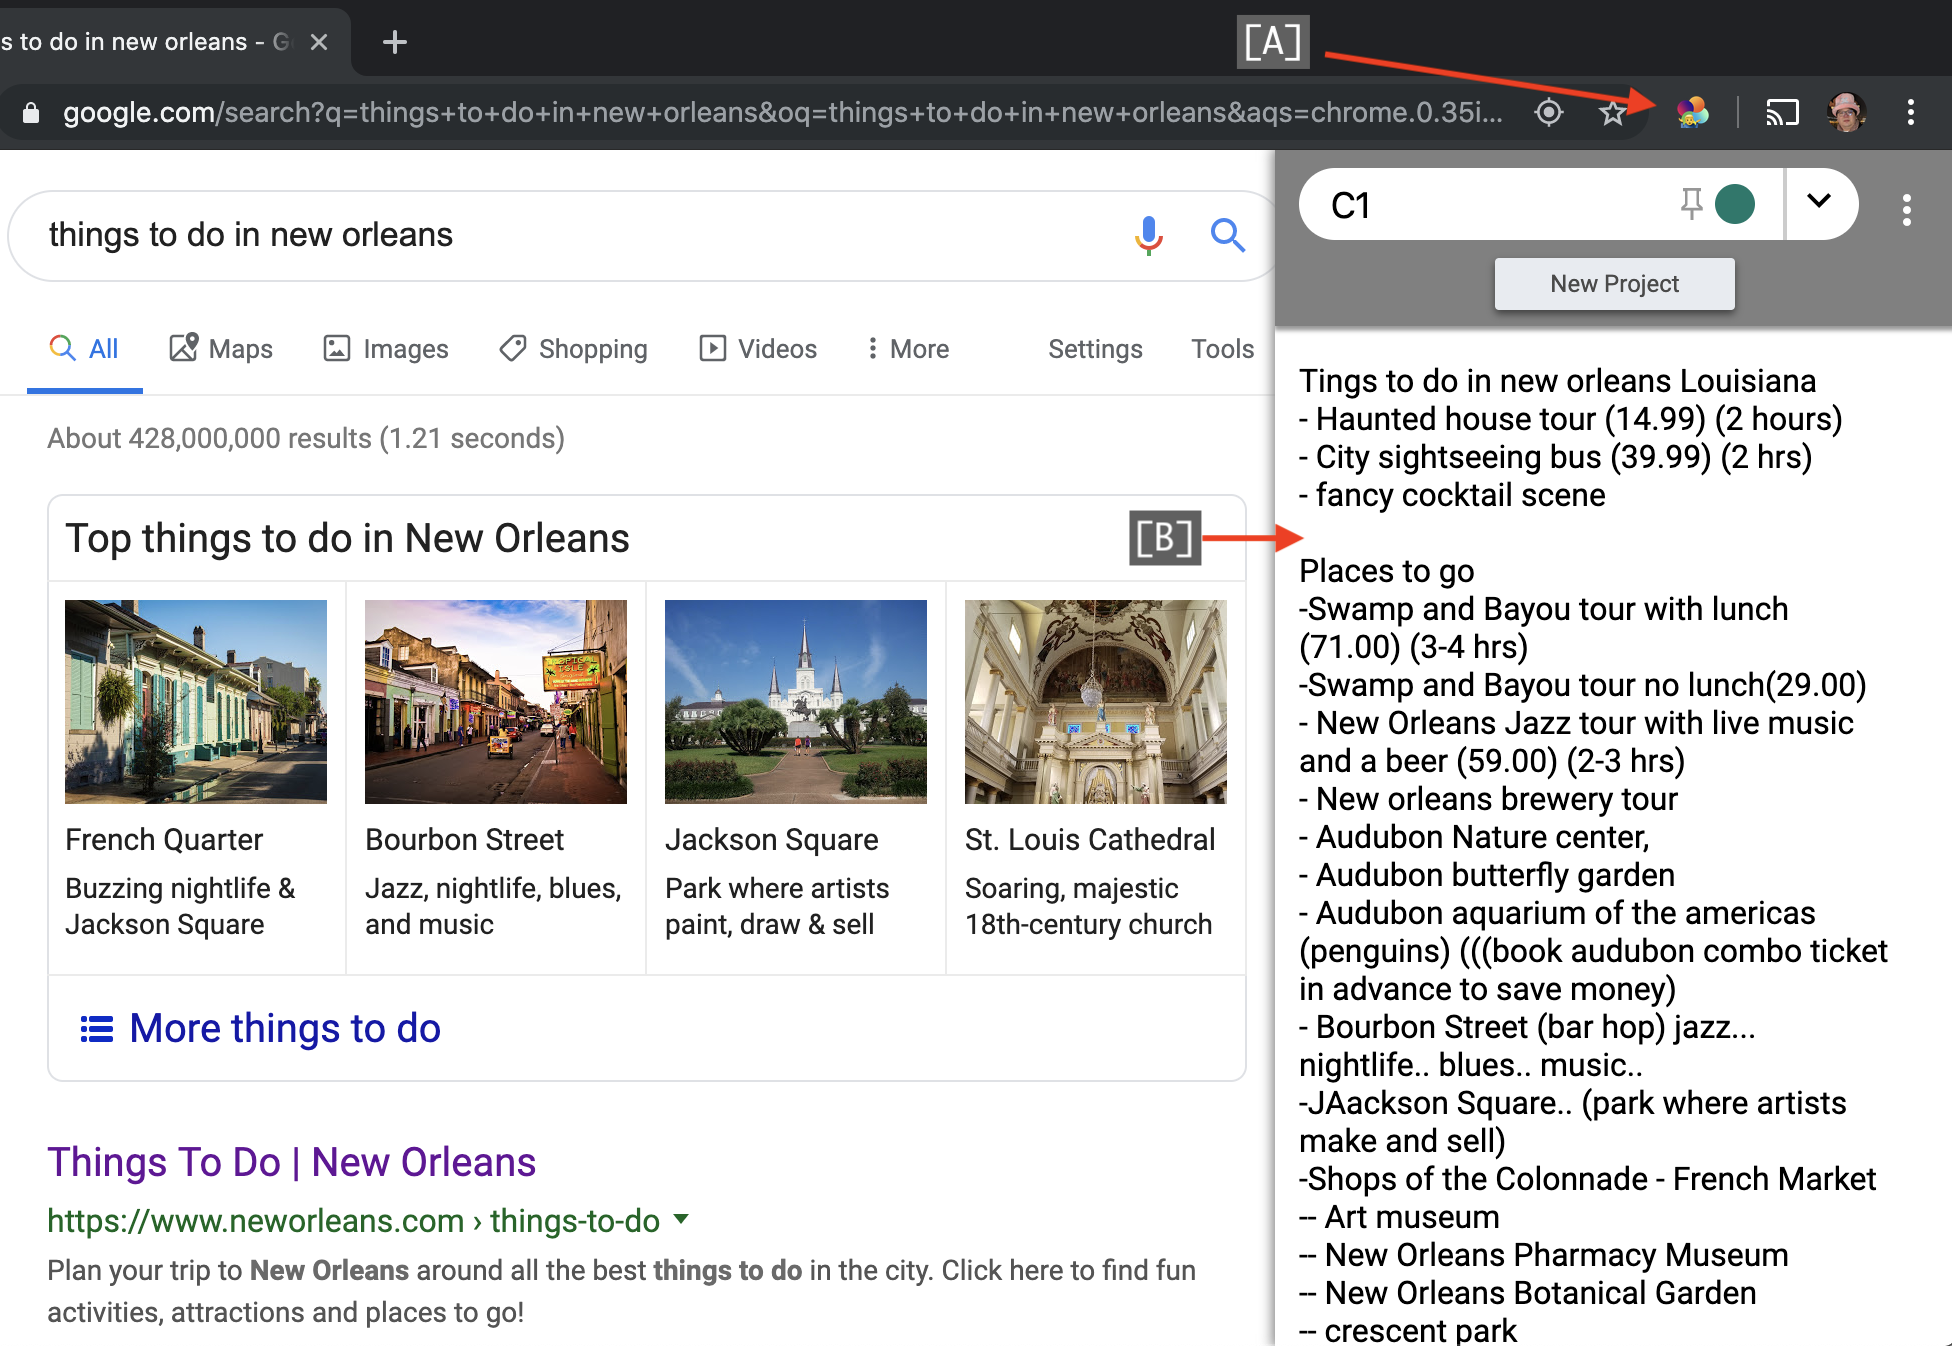
\includegraphics[width=1.0\columnwidth]{Chapters/Weaver/Baseline3.png}}
    \caption[One participant's project screenshot in the baseline variant of Weaver]{The notes of one participant using the baseline system at the end of the study. The sidebar [B] can be opened and closed on any webpages by clicking the extension button [A]. As participants typed into the sidebar, it is automatically saved and synced across browser tabs in real-time where the sidebar was opened.}
    \label{fig:baseline_fusion}
\end{figure}



\begin{table}
  \centering
  \scriptsize
% question, number of sources, number of clips, number of turkers
  \begin{tabular}{ l  r l   r l l }
  
	
    \textbf{ Behavior {\textbackslash} Systems} {\scriptsize(between-subject)} &
    	\multicolumn{2}{c}{\textbf{Weaver {\scriptsize(N=12)}}} &
    	\multicolumn{2}{c}{\textbf{Baseline {\scriptsize(N=12)}}} & \textbf{Independent-samples t-test}
    	\\
	
	\hline
	
	\# of webpages the system was accessed from &
    \textbf{12.00} & $\sigma$=~4.81 &
    \textbf{5.08} & $\sigma$=3.64 &
    $t(22)=+3.97,~~p < 0.001^{\tiny***}$ \\
    
%	&
	\# of webpages evidence was collected from &
    \textbf{5.33} & $\sigma$=~~2.58 &
    \textbf{3.40} & $\sigma$=1.89 &
    $t(22)=+2.45,~~p < 0.05^{\tiny*}$\\
    
    
%	&
	\# of evidence (notes{\&}clips) added to an entity &
    \textbf{18.42} & $\sigma$=12.65 &
    \textbf{6.50} & $\sigma$=5.38 &
    $t(22)=+3.00,~~p < 0.01^{\tiny**}$\\
    
%	&
%	\# of on-card metadata (e.g., addresses) added &
%	\multicolumn{2}{c}{\emph{not applicable}} &
%    \textbf{3.42} & $\sigma$=3.40 &
%    \\
    
%	A &
	\# of unique entities saved in the system &
    \textbf{8.92}  & $\sigma$=~6.49 &
    \textbf{13.42} & $\sigma$=5.94 &
    $t(22)=-1.77,~~p=0.09$\\
    
    \hdashline[1pt/1pt]

    
%	&
	\# of unique entity cards accessed by hovering &
    \textbf{29.33} & $\sigma$=15.62 &
    \multicolumn{3}{c}{\textit{}}
    \\
%	&
    \# of webpages each entity card was accessed from &
    \textbf{4.33} & $\sigma$=~1.40 &
    \multicolumn{3}{c}{\textit{entity cards were not available in baseline}}
    \\
%	&
	\# of times entity cards was accessed by hovering &
    \textbf{128.75} & $\sigma$=72.11 &
    \multicolumn{2}{c}{\textit{}}
    \\
    
	
	\hline
	
  \end{tabular}
  \caption[Evaluation results showed participants who used Weaver collected more evidence from more sources.]{Evaluation results for our primary domain of Travel Planning -- Mean statistics of participant behavior using Weaver and a Baseline system with an in-situ notepad. Results showed participant who used Weaver collected more evidence and from more information sources.}
  \label{tab:results_main}
\end{table}

\subsection{Implementation Detail}

Both Weaver and the baseline system were built as add-ons for the Google Chrome browser implemented in JavaScript using the ReactJS\footnote{https://reactjs.org} library. The application uses Google's Firestore real-time database\footnote{https://firebase.com} to store mappings between webpages and entities and user-generated notes and clips. To power the entity cards in Weaver, we utilize the Yelp Search API to fetch entities from Yelp, and we use the open-sourced DBpedia Spotlight \cite{spotlight} software in a custom backend that identifies DBpedia entities \cite{dbpedia} in webpages and syncs them with the end-user interface through the Firestore service. The studies were conducted using 12.5 inch Chromebooks running Chrome version 69, but both extensions were compatible with other operating systems where the Chrome browser is available.\footnote{The Chrome extension APIs are also currently being standardize by the W3C to be used across other browsers: https://www.w3.org/community/browserext/}

\subsection{Results}


%\subsection{Prior Domain Expertise}
%In terms of domain expertise, none of the 12 participants in our primary domain task reported having ever traveled to New Orleans, and conduct travel planning once to a few times per year or once in a few years (N=11, 1). However, we discovered that the camera task had very different characteristics for half of the participants who either strongly agreed or agreed that they \emph{understand what DSLR cameras are} versus 4 camera novices who did not agreed with the statement, using a 7-point Likert-scale where 1 indicates strong disagreement to 7 for strong agreement (Table~\ref{tab:results}; $\bar{x}$=6.75, 3.50, $\sigma$=0.5, 1.73).
%Based on reviewing their notes and saved cards, domain experts in general used Weaver to collect information about various camera models, while the novices largely spent their time reading to understand the various terminologies and differences between the two camera types listed in the task descriptions.
%Closer examination showed that the novices on average saved only around a third as many entity cards when compared to the experts (N=4, 4; $\bar{x}$=5.5, 15.25; $\sigma$=5.3, 2.9).
%Given the differences in prior knowledge and that the novices likely spent significant time on learning domain knowledge (i.e., DSLR and mirrorless cameras) and interacted less with Weaver's features, \textbf{we reported the two groups separately in Table~\ref{tab:results}, and focused our analysis on participants assigned our primary domain of travel and the expert participants in the camera task}. In the Limitations section, we will discuss the effects of prior domain knowledge and potential ways to address them. 
%In the results reported below, we report descriptive statistics around interactions where appropriate. 

Our main goal in designing Weaver is to support online sensemaking across different information sources.
Weaver supports this using two core mechanisms: \emph{Infusion} that allows users to access evidence about an entity scattered across other information sources, and \emph{Diffusion} that allows users to save supporting evidence about an entity to be resurfaced across other webpages that also mentioned the same entity. Through the two mechanisms, Weaver provides entity cards as a foraging structure where users can collect, reuse, and accumulate evidence from multiple webpages when evaluating a large number of options.

\subsubsection{Diffusion: Sensemaking across Webpages}

Results from our study in Table~\ref{tab:results_main} show participants who used Weaver interacted with the system more frequently than participants who used the baseline system. In addition, they also used Weaver to save nearly 3 times more evidences that were collected from significantly more webpages. On average, participants used Weaver on more than double the number of unique webpages compared to participants who used the baseline system (12.00 vs 5.08; N=12, 12; t(22)=3.97, p=0.0006 < 0.001$^{***}$).
In addition to accessing the system across more webpages, participants who used Weaver collected evidence (either by typing notes or copying clips) from more unique webpages. On average, each participant used Weaver to collect evidence from 5.33 different webpages ($\sigma$=2.58), which was significantly more than participants who used the baseline system who collected evidence from 3.40 different webpages based on an independent-samples t-test ($\sigma$=1.89; t(22)=2.45, p=0.02 < 0.05$^{*}$).
These results suggest participants used Weaver to better facilitate sensemaking across multiple webpages in the browser, allowing them to gather new information and access previously saved information across significantly more webpages.

Post-survey and interviews provided insights on how participants used the entity cards provided by Weaver to \emph{diffuse} and \emph{accumulate} evidence across webpages and used them to support decision making: 

\begin{tightquote}
``The cards were useful because they allowed me to add to things I found on other pages.
I could compound things that I had already said and supplement my knowledge to help me arrive at a decision.''
\end{tightquote}

On the other hand, participants assigned the baseline system pointed to the high interaction costs associated with saving evidence to their sidebars. Specifically, they described the tension between manually maintaining a useful organization in the sidebar and capturing all the useful information they had encountered:

\begin{tightquote}
``There were times I wanted to like highlight a passage, or save some text from a webpage [but didn't]... I was sort of using my notes as a TO-DO list, and sometimes I move things around to organize them. But if there are big blocks of text in there it'll be harder to do that, or even just to look at the list of things I have collected.''
\end{tightquote}

\noindent Conversely, participants who used Weaver described lowered interaction costs when saving information to the entity cards, as well as lowered interaction costs to remove all evidence related to an entity that later became irrelevant:

\begin{tightquote}
``I liked that I could save entities with notes attached and look back at them all put together. I used to do this with a word doc and links and it wasn't nearly as easy.''

``They [the entity cards] were very useful... I could save anything, and if I didn't need it later it was simple to erase them.''
\end{tightquote}

These findings suggest that the entity cards in Weaver were not only used as foraging structures to support sensemaking across multiple webpages, but also allowed participants to collect and synthesize evidence to support decision making with lowered interaction costs. As a result, we also found participants who used Weaver on average collected nearly 3 times more evidence compared to participants who used the baseline system (18.42 vs 6.50; t(22)=3.00, p=0.006 < 0.01$^{**}$).

\subsubsection{Infusion: Engaging with Entities during Browsing}

Traditional entity-centric approaches required users to interact with entities only during the retrieval stage, such as presenting entity cards in search engine results pages. While this approach improves efficiency for factual information needs, such as looking up the weather or the address of a restaurant, for complex exploratory search tasks, users have to consider many more opinions, facets and features about an entity, usually from a number of webpages. Our entity-centric approach explores the benefits of integrating rich entity information to stages beyond retrieval when conducting complex exploratory search tasks.

Our results show that Weaver participants were frequently engaged with the entity cards throughout the study. While participants in both conditions saved multiple entities to keep track of the different options that they were interested in, Weaver participants were actively evaluating potential options with information \emph{infused} from other webpages and external knowledge bases. Participants who used Weaver frequently accessed the entity cards by hovering over highlighted entity mentions on each webpages. On average, each participant who used Weaver hovered over entity mentions 128.75 times (Table~\ref{tab:results_main}; N=12, $\sigma$=72.11). We examined the number of entities participants saved in the two conditions. In Weaver, participants save entities by ``hearting'' an entity cards which also saves all the entity attributes that was on the card. In the baseline system, participants typed or copy-pasted the names of different entities into their sidebar, and would sometimes manually collect attributes that were readily available for participants who were using Weaver (such as addresses and Yelp review scores). At the end of the study, each participant on average saved 8.92 entities to Weaver ($\sigma$=6.49), which is slightly lower than participants who used the baseline system (13.42, $\sigma$=5.94), but the difference was only marginally significant based on an independent-samples t-test (t(22)=-1.77, p=0.09).

Even though participants who used Weaver did not save more entities to their workspace, they hovered over an average of 29.33 unique entities ($\sigma$=15.62) to access their entity cards throughout the study. In addition,
participants used Weaver to access the same entity cards while browsing different webpages. On average, each unique entity card was accessed from 4.33 different webpages ($\sigma$=4.33, N=12). This further indicates that participants who used Weaver not only collected evidence across multiple information sources for the options that they saved, they also relied on information from multiple information sources \emph{infused} to the entity cards to evaluate many potential options before saving them into their workspaces.

Post-survey and interviews showed that participants in both conditions relied on multiple sources to decide which entities to save in their workspaces: 

\begin{tightquote}
``There are like clear definite yeses that I would save immediately, but there's also a lot of maybes. For the maybes if I see something multiple times and they might get added.''
\end{tightquote}

\noindent Participants who used Weaver found value in the evidence automatically \emph{infused} from other webpages and external knowledge sources. Participants cited using information on the entity cards to verify uncertain or potentially biased information on the page that they were reading: 

\begin{tightquote}
``They [the information on entity cards] allowed me to see if the comments on this page was true''

``The cards were useful because I can know the exact condition other than the advertisements provided by their own company [referring to content on an official listing page].''
\end{tightquote}
 
These results show that entities served as options in the travel planning task, and that entities mentioned in text represented a useful structure for foraging across webpages. By identifying them in the browsers, participants were able to use the entity cards to keep track of interesting options and organize their notes and evidence collected from webpages about them.

Participants who used Weaver also pointed lowered interaction costs for managing additional browser tabs. They cited that the entity cards allowed them to better evaluate options encountered on the current webpage without the need to create to additional searches and managing additional browser tabs:

\begin{tightquote}
``I liked seeing similar material for an entity [referring to clips from different webpages] and being able to continue research without having to do an actual search.''

``They [the entity cards] were very useful when I needed to pull up information on something I tagged [saved], without the need to use multiple [browser] tabs...'' 
\end{tightquote}

\noindent These responses suggest that information \emph{infused} in the entity cards can help participants more confidently evaluate newly encountered options and used the entity cards to validate information presented on the current webpage.
Prior work pointed to the high cost of context switching for note taking can break the linearity of documents, and be disruptive for reading and consuming information \cite{chang2016supporting,tashman2011liquidtext,o1996towards}. Specifically, \cite{marshall1999introducing} found their participants intend to investigate other articles referenced by the current one, but avoided doing so in order to avoid disrupting their flow of reading of the current article.
The above responses in particular, suggested that the lightweight cross-referencing powered by the \emph{infusion} mechanism can potentially address this issue.

%Weaver also allowed participants to accessed the same entity cards through its mentions across webpages. On average, each participant examined 29.33 ($\sigma$=15.62) unique entity cards (Table~\ref{tab:results_main}), and each entity card was called out via hovering over their mentions on 4.33 different webpages ($\sigma$=1.40). This suggests that participants were using a set of entity cards of interests to evaluate their options when browsing different webpages.

Surprisingly, participants also mentioned discovering and navigating to useful information sources from examining information on the entity cards, which was not our original design intention:

\begin{tightquote}
``[It was useful when] I was taken to mentions on sites I would not have thought of''

``[entity cards] Give you info about other websites that might be useful later on.''
\end{tightquote}


%\noindent At the same time, other participants also described how they would prefer to use information sources that were familiar and trusted to them (such as TripAdvisor) instead of webpages returned from search engines. This suggests a future direction for personalizing the entity cards to prioritize sources already trusted by the user.

These results showed that participants were actively engaged with the entity cards in the Weaver system, and that bringing entity support beyond search results pages to support active reading and note taking can also be beneficial for users using multiple information sources to conducting online sensemaking. In addition, participants also found value in the mentions of entities \emph{infused} from multiple webpages, using them as context to evaluate both their entity options as well as potentially biased information on the current webpage.



\section{Discussion}

\subsection{Limitations and Generalization}

In this work, entities were used as a proxy for potential options in complex sensemaking tasks. This allowed us to exploit state-of-the-art entity linking algorithms to automatically identify and disambiguate entity mentions in plain text across webpages and users' notes. While we believe entity-centric search can cover a wide variety of tasks -- past work has shown entity focused queries account for the majority of search traffic \cite{guo2009named,lin2012active} -- there are still scenarios where potential options can be topical or descriptive. For example, potential options for ``How do I get my tomato plants to produce more tomatoes?'' could include \emph{fertilization}, \emph{pruning}, and \emph{providing proper support} as shown in \cite{ka,alloy}, which can potentially be supported using micro-interaction driven structuring approaches \cite{alloy,hu2014interactive}.

%One common theme was the lack of support for capturing structured entity attributes from webpages, such as multimedia or addresses especially when manually creating an entity card that was missing from the system (Figure~\ref{fig:custom}):

%\begin{tightquote}
%``Easy to make a record, but not easy to record all the information I need, such as addresses and photos.``

%``[Improve Weaver so I can] Mark the address on Google map if a place doesn't have an existing map location.'' 
%\end{tightquote}

%\noindent Future work could involve providing better support for extracting structured information from webpages. For example, looking at alignment between DBpedia information and information on the page, or structured information extraction from webpages through end-user interaction \cite{thresher,bier2006entity}.

With the ability to recognize options for entity-based tasks, Weaver focused on allowing users to gather and synthesize evidence across webpages about each of their options. On a higher level, Weaver provided a simple category structure for organizing multiple saved entity cards, but participants also pointed to the need for further synthesizing their collections of cards in the later stages of sensemaking:

\begin{tightquote}
``Weaver is helpful in the first stage of information collection, but when it comes to the final detailed plan of the trip, I still need more place for editing, adding specific time and so on.''
% Also I need to access my plan through my phone, so the calendar or memo are more useful during the trip.
\end{tightquote}

\noindent This suggests that more detailed artifacts that leverage these entity-centric cards, such as a calendar for itineraries, could be an promising next step.

%This includes writing out a travel itinerary using a word processor or calendar software, and also accessing collected information on mobile platforms:


%\subsubsection{Supporting Other Domains}

%In a small pilot study, we explored the potential costs of generalizing Weaver to a different domain using a DSLR camera shopping task:

%\begin{tightquote}
%A friend is asking for your help to figure out what DSLR and mirrorless cameras are and which model she should buy as a beginner.
%\end{tightquote}


%\noindent Unlike the travel planning task, the current implementation of Weaver does not have a knowledge base specialized for camera products, and most webpages in this task do not contain any geographic entities. In addition, this camera shopping task also involved significant learning and expertise with concepts and terms that might be unfamiliar.

%We followed the same study protocol and recruited 8 participants who had different levels of prior domain knowledge. In the pre-survey, four expert participants self-reported that they understood or were familiar with what DSLR cameras are, while the other four novice participants did not.
%In theory, Weaver could help novices with general knowledge-building using information from DBpedia by allowing users to quickly look up the definition of unfamiliar terminologies and concepts using the entity descriptions from DBpedia, such as ``aperture sizes'' or ``CMOS sensors''. Based on behavior logging and post interviews, expert participants  utilized Weaver in similar ways to participants in the main travel study, using entity cards for different camera models to keep track of potential options and to collect evidence from multiple webpages.
%In contrast, the novice participants largely spent their time reading to understand the various terminologies and differences between the two camera types listed in the task descriptions. However, they did not find the short description extracted from Wikipedia sufficient for this purpose. This suggests that the current implementation of Weaver is more beneficial for the evidence gathering and deciding stages of sensemaking compared to early learning, although it is possible that with knowledge bases more appropriate for learning general knowledge in the target domain, an entity-centric approach might still be beneficial.

%Participants who were novices in the domain would need to first learn the technical terms and domain knowledge in cameras and photography before advancing to the stage where they can evaluate different options (i.e., camera models) to collect evidence.
%For example, helping novice participants to understand and take notes about unfamiliar technical terms (e.g., full-frame CMOS sensors) using entity cards from DBpedia. We chose these characteristics to probe the application of an entity-centric approach in a situation where there might not be good coverage of entities and attributes, and where some users might not have the required domain knowledge to evaluate the different options in webpages. 

%Participants also pointed to issues they encountered during the study, which inform ways to improve future versions of Weaver so it can be adopted by a wide range of domains and scenarios.


%\noindent Similarly, participants in the camera shopping task cited the high cost of capturing camera specifications:

%\begin{tightquote}
%``The cards did not provide any additional information about the cameras. However, they were useful in keeping track of the features of different cameras.''
%\end{tightquote}

%This potentially explains the higher number of saved notes for participants in the camera task. While DBpedia actually contains detailed specifications of many DSLR camera models,\footnote{http://dbpedia.org/page/Canon\_EOS\_750D} entities in DBpedia typically have dozens to hundreds of attributes. Weaver only surfaced the most common attributes (i.e., location, short description, and categories) so it does not overwhelm users.

%\begin{tightquote}
%``Mkbhd [Marques Brownlee, a popular YouTuber] and others are good tech reviewers and they can provide a better pro vs con list than reading [the mentions].''
%\end{tightquote}



\subsection{Conclusion and Future Work}

In this paper we introduced Weaver, a novel approach for weaving together information about entities that were scattered across the Web to support complex sensemaking in the browser. By presenting in situ entity cards, users can both verify potentially biased information on the current webpage with evidence \emph{infused} from other sources, as well as using the entity cards as foraging structures that can \emph{diffuse} their notes across browser tabs and be resurfaced automatically as they become relevant. In a lab study with 24 participants, we compared Weaver to a baseline system with no entity support as a between subject condition. We observed that participants using Weaver gathered nearly 3 times more evidence from 60\% more webpages, both significantly more than participants who used the baseline system. Post-interviews revealed how they utilized Weaver to verify information they encountered, to accumulate evidence across webpages, and to synthesize them to support decision making.

%We chose a holistic evaluation despite it required us to implement a relatively complete set of features, because we believed we would learn more from testing the end-to-end system in more realistic sensemaking scenarios as opposed to trying to isolate individual interactions. For example, an earlier version of Weaver did not include maps and the overview page. This led to participants maintaining the entities cards in Weaver and a separate Google Maps project to figure out their proximity to each other. As a result, participants viewed the earlier version of the system as incomplete, and some responded that they were spending significantly more effort than their current practice of using Google Maps as their primary trip planning tool.
%Early testing also uncovered that showing all cards detected in the viewport immediately in the sidebar was too intrusive during complex sensemaking tasks. As a result, we switched to the current design of only showing an entity card when its underlined mentions were hovered on, which was much better received. While we used simple highlighting with different colors to indicate an entity mention has additional information and whether the same entity was interacted with before, in situ visualization techniques (such as \cite{hoffswell2018augmenting}) can also be explored for annotating webpages with richer information. 

%Evaluation results showed that participants valued both Infusion- and Diffusion-based features, and were actively using the Weaver system to gather more evidence from significantly more information sources when compared to the baseline system. However, we also learned that adoption may be critically sensitive to the cost structure of extracting entities and attributes. Some limitations identified by our participants can potentially be addressed with approaches in previous work. For example, using end-user interactions to bootstrap entity-attribute extractors \cite{thresher,bier2006entity}.

%Prior work that also used an in situ note taking interface found their participants rarely re-access previously saved notes \cite{notetoself}. However, in our study, we observed that our participants were frequently engaged with the same entity cards when they read different webpages, and used them to accumulate and compound evidence and notes. This suggests that our entity-centric approach offers a potential solution for re-accessing via automatically resurfacing previously saved notes as they became relevant to what the users were reading (i.e., when they mentioned the same entities). Further investigations are still needed to understand the longer term effects of this mechanism beyond the 50 minute sensemaking task in our lab study.

%During development, we also considered several different ways in which entity cards might be surfaced to provide context to users. In the first version of Weaver, we detected which entities were mentioned in the browser viewport and displayed a list of entity cards in the overlay. Our intention in exploring this design was to provide a visual trigger for users to learn about the context of entities and potentially act on that context by annotating or saving relevant entities. However, participants in our preliminary user studies raised the issue that many of the entities surfaced were not relevant to their tasks, and having to sift through the list of entity cards and locate relevant entities was time consuming. Many of these irrelevant entities were either overly general locations (e.g., U.S.A), ambiguous or partial matches (e.g., ``park''), or general knowledge entities from Wikipedia (e.g., Cuisine of the Southern United States). While it is possible that approaches taking into account the user's prior knowledge about the task and their query intent might improve the relevance of returned results (e.g., \cite{pasupat2014zero}), the density of entities within the browser viewport constitutes a more fundamental issue that leads to cluttering the browser interface and overwhelming users with too much information at once \cite{wilson2008improving}. Based on these observations, we changed the interface to highlight recognized entity mentions and allowing users to query for entity cards that they determined to be relevant by hovering over the mentions.

We think entity-centric approaches have the potential to support sensemaking in a wide variety of domains that involve collecting evidence and deciding between options. However, the cost of adapting the current framework to support different domains is unclear, especially for domains where high quality knowledge bases are not readily available. In the post-survey, we asked participants if they could think of other search tasks that may benefit from using Weaver, and participants pointed to a variety of different tasks, including making a purchasing decision, essay writing, event planning, literature review, job searching, and deciding on a college major. Here we describe scenarios to illustrate how the infusion/diffusion framework might work for two of these tasks.

\begin{itemize}
    \item A researcher can create a ``paper card'' (using Microsoft Academic Graph for metadata) to externalize ideas as she reads a paper and create additional cards for ideas relating to cited papers, providing a foraging and ideation structure during literature review where papers may have overlapping citations. 

    \item A consumer can create ``product cards'' for different cameras (using online shopping APIs for pricing info and DBPedia for specs) to keep a ``short list'' as they compare different options by collecting both objective and subjective info in reviews relevant to her personal needs. In this case, users can also configure Weaver to focus on only cameras entities to improve linking and disambiguation performance.
\end{itemize}



Finally, we also see promise in a number of other research directions. One such direction would be automatically summarizing evidence gathered across different websites for an entity instead of simply listing them. This could help Weaver scale to much larger projects with many sources, while keeping gathered information easy to consume for the users. However, surfacing information sources in the summary so users can better evaluate source trustworthiness is still an open problem. While Weaver supported synthesizing entities and evidence into categories, providing support for creating different structures (e.g., tables or essays) warrants further investigation.

Our results have implications for the design of future intelligent browser interfaces that can better understand the information being consumed by their users, and building novel interactive systems for supporting online sensemaking. While there are already popular commercial browser add-ons that allowed users to collect information from webpages with lowered efforts (such as Evernote Web clipper), almost all existing tools require users to switch to a separate workspace to access saved information. Our findings pointed to benefits in better integration between collecting information from webpages and accessing them.
As phenomena such as fake news and shill reviews have demonstrated, there are significant drawbacks to the easy availability and generation of online content. Interactive systems that can provide additional context to users \emph{in situ} may become increasingly necessary to help navigate the information overload. Anecdotal evidence for this need can also be seen in the rise of aggregation-based sites such as Metacritic or Wirecutter, which act as virtual meta-analyses of evidence and opinions but fail to take into account the personal context of the user and their goals. We believe that this work presents a step forward in illustrating a design space for interactive systems which can take advantage of advances in machine learning and natural language processing to help end users actively gain context and personalize their online sensemaking experience.


%\section{Conclusion} %(or remove the below)
%We introduced Weaver, a browser add-on that enable the browser to better understand information consumed by its users for supporting sensemaking across webpages while conducting complex exploratory search tasks. Traditional approaches for supporting exploratory search tasks either try to generate better search results page or with an external interface for organizing saved information. We instead use an entity-centric approach to support the process of collecting and organizing evidence from multiple information sources. Weaver empowers users to better evaluate entities with relevant information ``infused'' from other webpages, and allows users to ``diffuse'' their notes about an entity across different webpages where the same entity was mentioned. In our user study about trip planning, participants valued both Infusion-based and Diffusion-based features, and considered Weaver an improvement to their current practices.

